\chapter{Conceitos básicos}
\label{cap:structure-of-speech}

Nesta seção, abordaremos uma parte teórica do reconhecimento automático de voz. Muitos dos conceitos citados serão importantes para melhor entendimento e implementação do módulo posteriormente.

% ---------------------------------------------------------------------

\section{Definição de reconhecimento de voz}

% https://en.wikipedia.org/wiki/Speech_recognition
% https://en.wikipedia.org/wiki/Computational_linguistics

\textit{Reconhecimento automático de voz} (ou da fala), ou \textit{speech to text} (STT), é um campo multidisciplinar que envolve as áreas de Inteligência Artificial, Estatística e Linguística. Busca-se desenvolver metodologias e tecnologias para que computadores sejam capazes de captar, reconhecer e traduzir a linguagem falada para texto.

% https://www.nap.edu/read/19357/chapter/4#10
\begin{figure}[H]
  \centering
  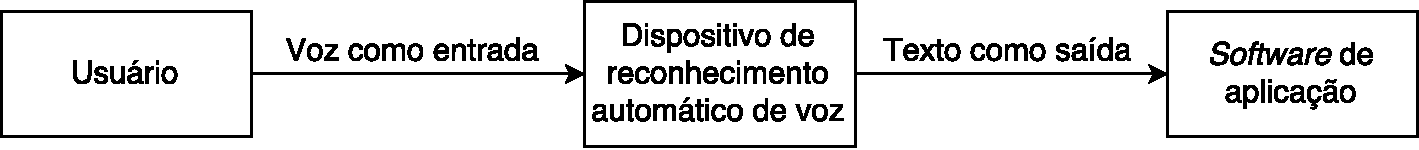
\includegraphics[width=.7\textwidth]{image/speech_system.pdf}
  \caption{Sistema genérico de reconhecimento automático de voz}
  \label{speech_system}
\end{figure}

% ---------------------------------------------------------------------

\subsection{História e aplicações}

% https://nexbridge.co.uk/speech-recognition-in-the-21st-century/
% https://www.callcentrehelper.com/the-top-five-uses-of-speech-recognition-technology-1536.htm
% http://www.pcworld.com/article/243060/speech_recognition_through_the_decades_how_we_ended_up_with_siri.html
O primeiro sistema de reconhecimento de voz conhecido foi o \textit{Audrey}, construído em 1952 por três pesquisadores do \textit{Bell Labs} para reconhecer dígitos falados por um único usuário. 10 anos depois, a IBM apresentou a máquina \textit{Shoebox}, que reconhecia 16 palavras em inglês.

Sistemas de reconhecimento de voz só tiveram um avanço realmente significativo na década de 80, devido a um método estatístico denominado \emph{modelo oculto de Markov} (HMM, sigla para \textit{Hidden Markov Model}). Ao invés de procurar por modelos de palavras em padrões de som, HMM considerava a probabilidade de um som desconhecido possuir palavras, o que acelerou o processo e tornou possível usar um vocabulário maior nos computadores. Outro modelo que ganhou bastante popularidade na época foi o de redes neurais, que é efetivo para classificar palavras isoladas e fonemas individuais mas encontra problemas em tarefas envolvendo reconhecimento contínuo. Ao contrário do HMM, este método não consegue modelar bem dependências temporais.

A evolução na tecnologia de reconhecimento de voz foi tamanha que, atualmente, é inegável seu impacto em nosso dia a dia. Um celular moderno consegue captar palavras ou pequenas frases de seu usuário dentre um enorme vocabulário para fazer buscas na Internet, tocar uma música ou fazer uma ligação. Muitas empresas utilizam máquinas para receber ligações de seus clientes; de acordo com o que interpretam, a chamada é redirecionada para um funcionário mais adequado. Alguns países chegam até a usar reconhecimento de voz para autenticar a identidade de alguém por telefone, com o objetivo de evitar fornecer dados pessoais pelo mesmo. Também há usos em transportes, na área médica e para fins educativos.

% ---------------------------------------------------------------------

\subsection{Sistemas dependentes e independentes}

% https://speechangel.com/2016/05/04/difference-speaker-dependent-speaker-independent-recognition-software
% http://www.voice-commands.com/103.htm
Existem duas variantes de reconhecimento de voz:

\begin{itemize}
\item Os sistemas \textbf{dependentes} (\textit{speaker-dependent}), caracterizados pelo \emph{treinamento} feito pelo usuário. Isto é, são computadores que analisam e se adaptam aos padrões particulares da fala captada, resultando em uma maior acurácia. Geralmente, o usuário deve ler algumas páginas de texto para a máquina antes de começar a usar o sistema. Esta variante é comumente usada em casos particulares, onde um número limitado de palavras deve ser reconhecido com bastante precisão.

\item Os sistemas \textbf{independentes} (\textit{speaker-independent}), que são desenvolvidos para reconhecer a voz de qualquer pessoa e não requerem treinamento. É a melhor opção para aplicações interativas que usam voz, já que não é viável fazer com que os usuários leiam páginas de texto antes do uso. Sua desvantagem é a acurácia menor se comparado ao reconhecimento dependente; para contornar isso, costuma-se limitar o vocabulário reconhecido pelo sistema.
\end{itemize}

% ---------------------------------------------------------------------

\section{Estrutura da fala}

% ---------------------------------------------------------------------

\section{Modelo oculto de Markov}
